\begin{figure*}[ht]
\centering
    \begin{subfigure}[b]{0.52\textwidth}
            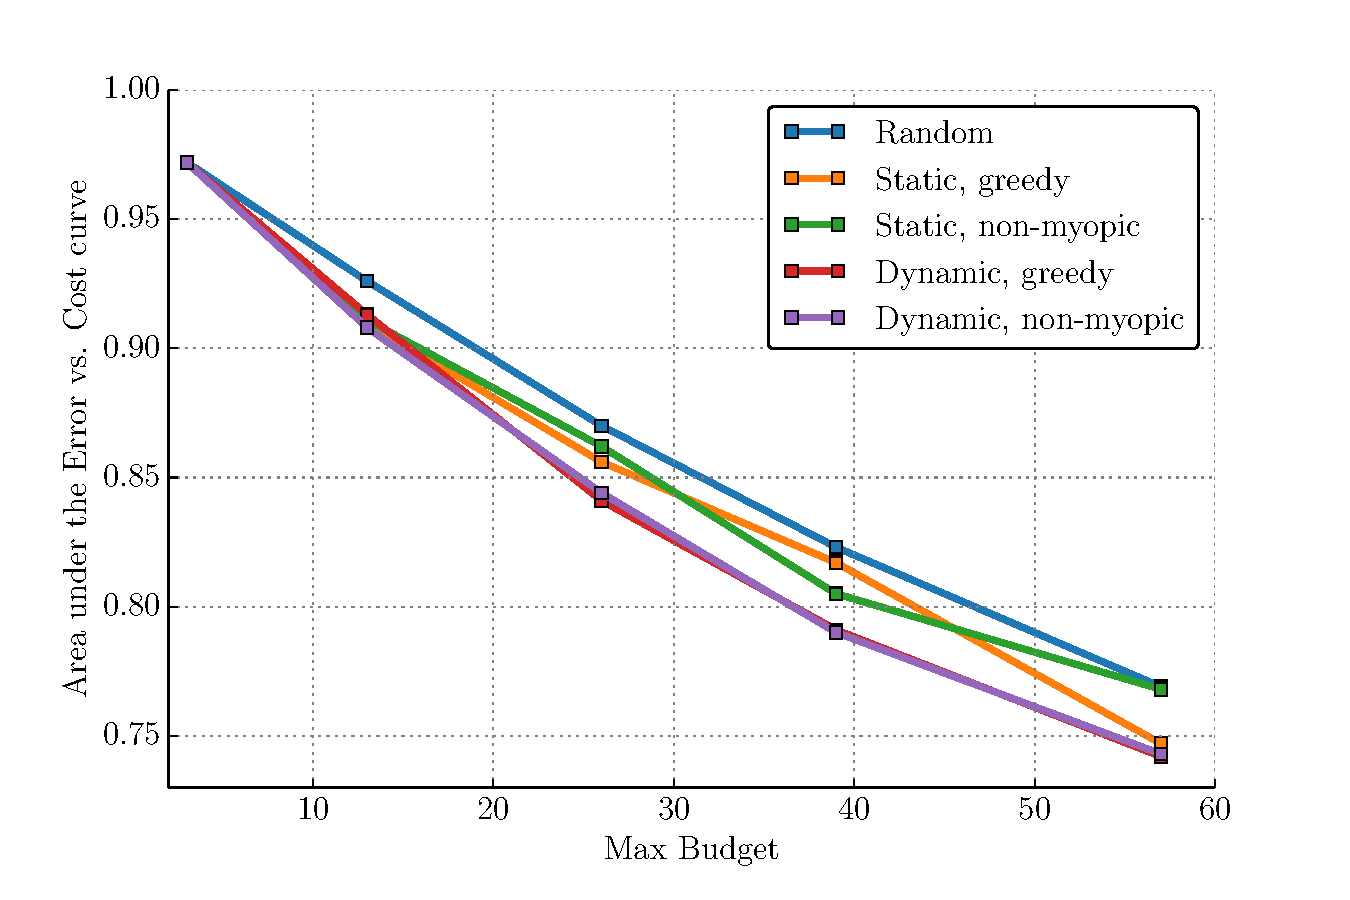
\includegraphics[width=\textwidth]{../../figures/apr11_assembly/_ilsvrc65_auc.pdf}
            \caption{
            Areas under error vs. cost curves for policies learned at different budgets.
            (No specificity back-off is performed here).
            \label{fig:imagenet-a}
            }
    \end{subfigure}\hfill%
    \begin{subfigure}[b]{0.43\textwidth}
            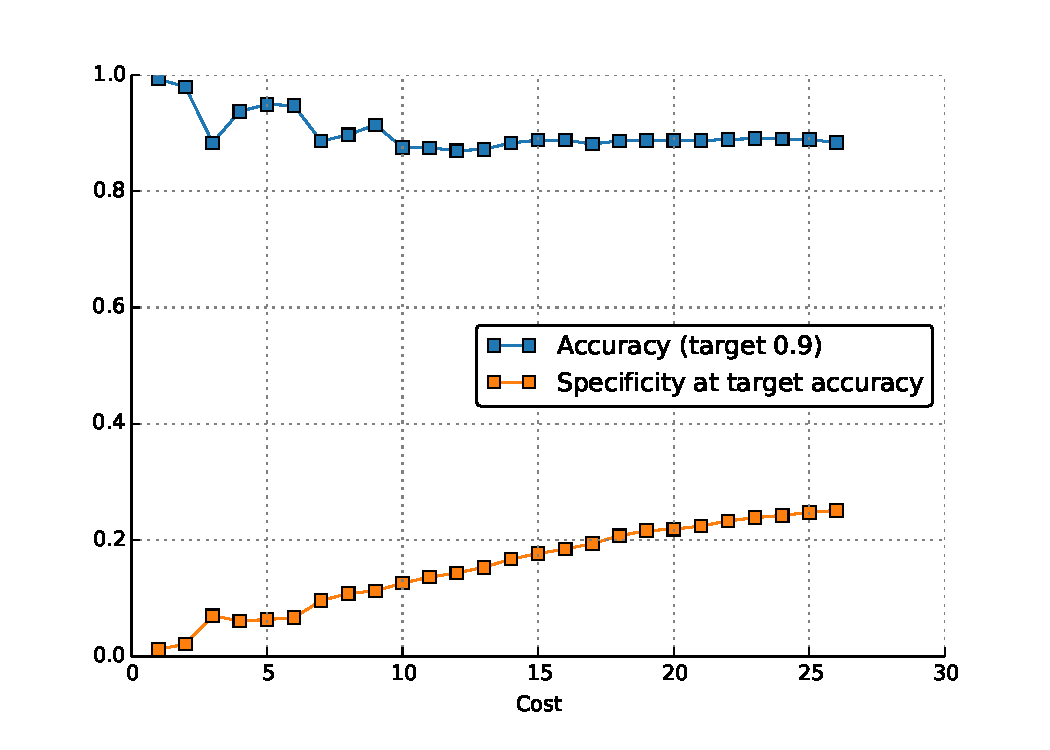
\includegraphics[width=\textwidth]{../../figures/apr11_assembly/ilsvrc65_acc.pdf}
            \caption{
            Holding prediction accuracy constant, we achieve increased specificity with increased cost (on \emph{Dynamic, non-myopic} policy, budget = 36).
            \label{fig:imagenet-b}
            }
    \end{subfigure}\\\vspace{1em}
    \begin{subfigure}[b]{.97\textwidth}
            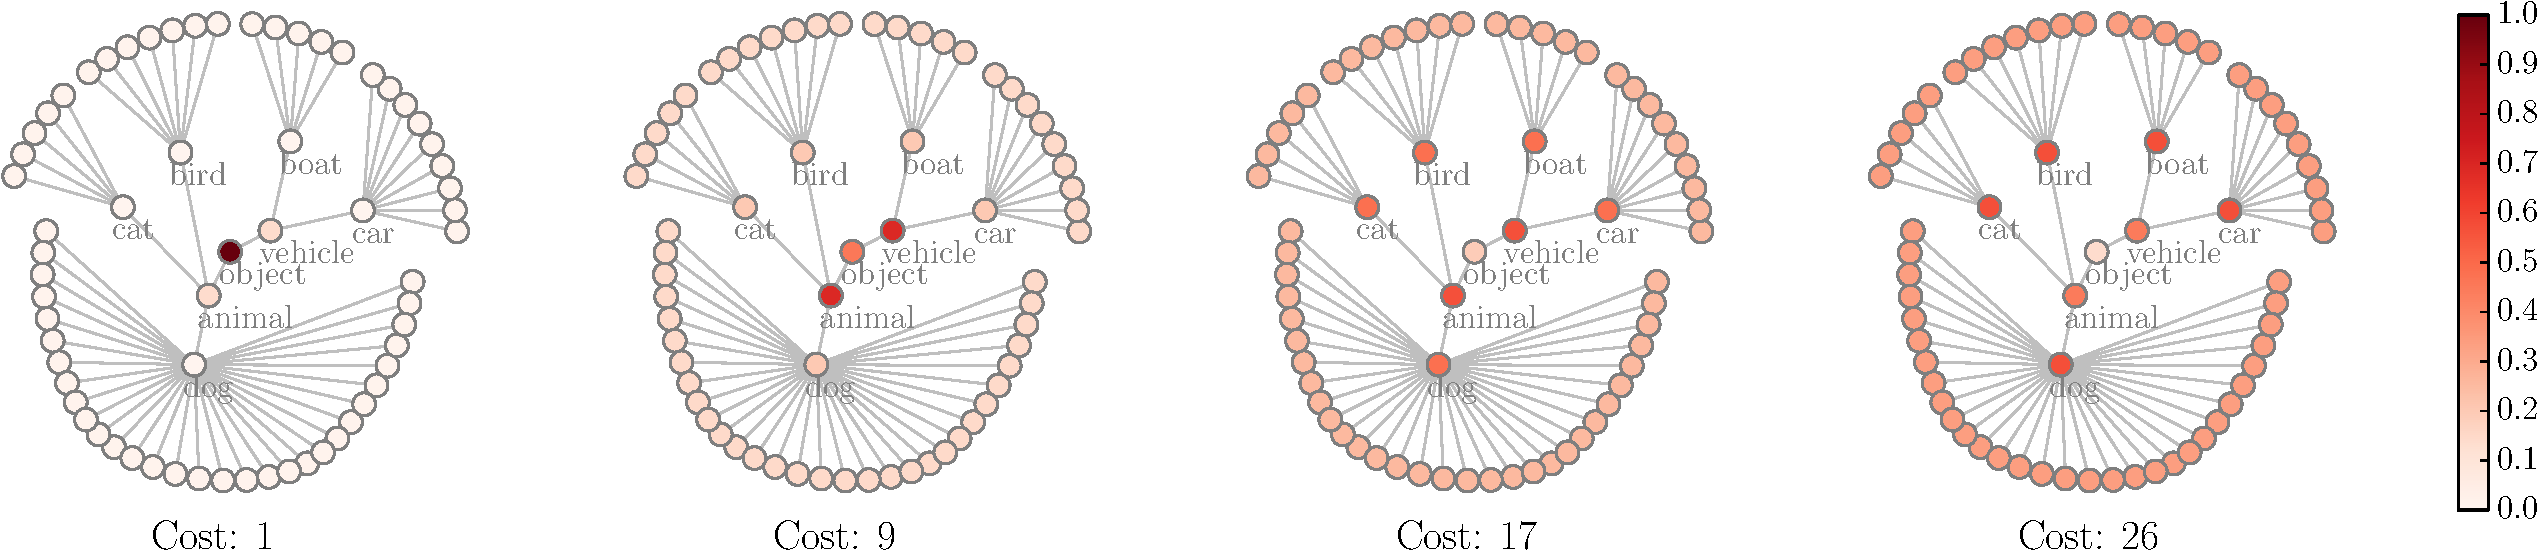
\includegraphics[width=\textwidth]{../../figures/apr11_assembly/ilsvrc65_network-crop.pdf}
            \caption{
            We visualize the fraction of predictions made at inner vs. leaf nodes of ILSVRC-65 at different cost points of an Anytime policy: with more computation, accurate predictions are increasingly made at the leaf nodes.
            \label{fig:imagenet-c}
            }
    \end{subfigure}
\caption[Results of the classification approach on the ILSVRC-65 dataset.]{
Results on the ILSVRC-65 dataset (best viewed in color).
Figure (a) shows our dynamic approaches outperforming static baselines for all practical cost budgets.
When our method is combined with Hedging Your Bets \parencite{Deng-CVPR-2012}, a constant prediction accuracy can be achieved at all points in the Anytime policy, with \emph{specificity} of predictions increasing with the cost of predictions.
Figures (b) and (c) show this for the \emph{dynamic, non-myopic} policy learned for budget = 26.
This is analogous to human visual performance, which shows increased specificity at longer stimulus times.
}\label{fig:imagenet}
\end{figure*}
